\chapter{User documentation}
\label{ch:user}

This chapter explains how to run AK\&VEN and how each kind of user works with it: the visitor and the customer in the
shop (Section~\ref{sec:shop}), and the staff, the owners and the super admin in the administration
(Section~\ref{sec:admin}). The screenshots show the demo catalogue in English; every screen is also available in
Russian and Kyrgyz.

\section{System requirements}

\subsection{Server}
\begin{itemize}
	\item Docker with Docker Compose~\cite{docker} (on macOS, Docker Desktop or Colima; on Linux, Docker Engine);
	\item about 2~GB of free memory and 3~GB of disk space for the images and the database;
	\item for the optional language model: an API key of a provider with an OpenAI-compatible chat API (Gemini by
	default) and outbound internet access.
\end{itemize}

Without Docker, the backend needs Java 17 and Maven 3.9, the frontend Node.js 22, and the data PostgreSQL 16 with the
pgvector extension; the developer documentation (Section~\ref{sec:running}) describes that setup.

\subsection{Client}
Any current browser (Chrome, Edge, Safari, Firefox) on a phone, tablet or computer. The shop can be installed as an
app from the browser's menu (``Add to Home Screen'' or ``Install''); once installed it opens in its own window and the
bag keeps working without a connection. JavaScript must be enabled.

\section{Installation and start}
\label{sec:install}

From the project folder, one command builds and starts the database, the backend and the web server:

\begin{lstlisting}[language=bash, caption={Starting the shop}, label=src:start]
docker compose up --build
# then open http://localhost:8081 in a browser
\end{lstlisting}

The first build takes a few minutes. The backend has started when its log ends with
\texttt{Successfully applied 35 migrations}; the database tables are created and, in the demo, filled with the
catalogue. To start again from an empty database, run \texttt{docker compose down -v} and start again.

\subsection{Demo accounts}
\begin{table}[H]
	\centering
	\begin{tabular}{l l l}
		\toprule
		\textbf{Role} & \textbf{Email} & \textbf{Password} \\
		\midrule
		Super admin & \texttt{superadmin@akven.test} & \texttt{changeme-super} \\
		Owner & \texttt{admin@akven.test} & \texttt{changeme-admin} \\
		Staff & \texttt{staff@akven.test} & \texttt{changeme-staff} \\
		Customer & \multicolumn{2}{l}{create one with Sign in, then Create an account} \\
		\bottomrule
	\end{tabular}
	\caption{Demo accounts}
	\label{tab:demo}
\end{table}

These accounts exist only in the demo. On a real installation the first super admin is created from the
environment, and the demo accounts are switched off at every start.

\subsection{Configuration}
\label{sec:config}

Settings are read from environment variables, usually from a file \texttt{.env} next to
\texttt{docker-compose.yml} (an example is in \texttt{.env.example}). None of them is required for the demo.

\begin{table}[H]
	\centering
	\begin{tabularx}{\textwidth}{l X}
		\toprule
		\textbf{Variable} & \textbf{Meaning} \\
		\midrule
		\texttt{SUPER\_ADMIN\_EMAIL}, \texttt{\_PASSWORD} & The first super admin of a real installation; switches the demo
		accounts off. \\
		\texttt{DEMO\_ACCOUNTS=on} & Keeps the demo accounts for a presentation. \\
		\texttt{LLM\_API\_KEY}, \texttt{LLM\_MODEL} & Lets a language model answer the chat (Gemini by default). \\
		\texttt{SHOP\_CONTACTS} & The family's real phone numbers and messengers, kept out of the repository. \\
		\texttt{JWT\_SECRET} & Optional signing key for logins; without it each installation creates its own. \\
		\texttt{CORS\_ALLOWED\_ORIGINS} & The web addresses allowed to call the API from a browser. \\
		\bottomrule
	\end{tabularx}
	\caption{The main settings}
	\label{tab:config}
\end{table}

\section{The shop}
\label{sec:shop}

\subsection{Everywhere: the header, languages, currencies and the footer}

The header holds the shelves (Shop, Men, Women, Kids, Gift Sets, Our Story), the logo, a Wholesale button, and icons for
the stall, search, saved socks, the account and the bag. The bar above it switches the currency (US dollars, Kyrgyz som,
Russian roubles, converted at the owners' rates), the language (EN, RUS, KYR, the last two written in Cyrillic) and light or dark colours. The whole site,
including messages from the server and the assistant's answers, follows the chosen language. On a phone the shelves
move into a menu.

The footer (Figure~\ref{fig:footer}) answers the last questions a visitor has: whether the stall is open right now (the
sign on container 70-E reads open or closed in Bishkek time), the address with links to Google Maps and 2GIS, how
pickup, delivery and payment work, every page grouped, the contacts, and a link to the privacy page, which explains in
plain words what the shop keeps and why.

\shot{u-footer.jpg}{The footer: the stall's door with its open or closed sign, the promises as sewn labels, every page and the contacts}{fig:footer}

\subsection{The home page}

The home page (Figure~\ref{fig:home}) opens on the socks: a still life of the everyday colours in an AK\&VEN box, two
buttons and the facts that matter. Below follow the four shelves as washing lines on their own fabrics
(Figure~\ref{fig:shelves}), the newest socks, the price ladder, the fitting room, what families say, a gift box, the
family planner, the story of the two names, and a short scene in which container 70-E opens as the visitor scrolls.

\shot{u-home.jpg}{The home page}{fig:home}
\shot{u-home-shelves.jpg}{Shop by who it is for: each shelf on its own fabric, with its socks on the line}{fig:shelves}

\subsection{The shelves: browsing and filtering}

A shelf (Figure~\ref{fig:catalog}) opens on its fabric with its socks pegged on the line and a tag with the number of
products. The tabs switch between all socks, men, women, children and gift boxes. The owners' sections are drawn as
occasions (Classic, Casual, Sport, Thermal, Home, Heritage); below them, a bar that stays in reach while scrolling
filters by height (no-show to knee-high), by size and by colour, shows only socks in stock and sorts by newest, name or
price. Every number on a filter says how many products it would leave; a choice that would leave none is disabled. Each
chosen filter appears as a tag that removes it with one tap (Figure~\ref{fig:filters}). The list grows twelve at a time
with \emph{Show 12 more}, and a thread shows how much of the shelf has been seen. Everything is kept in the address, so
a filtered shelf can be bookmarked, shared or reached again with the Back button.

\shot{u-catalog.jpg}{The men's shelf}{fig:catalog}
\shot{u-catalog-filters.jpg}{Occasions, heights, sizes and colours; the chosen size shown as a tag}{fig:filters}

On every card the heart saves the sock, and \emph{Quick view} lets the visitor choose a colour and a size and add it to
the bag without leaving the shelf.

\subsection{A product}

The product page (Figure~\ref{fig:product}) shows the pictures (the picture follows the chosen colour), the name, the
price, the colours and sizes, the honest stock (in stock, only a few left, arriving in about $n$ days, or sold out with
\emph{Tell me when it's back}), the quantity and \emph{Add to bag}. Under them come when the order can be collected, the
delivery countries and the collection discount, then \emph{How the price falls} (Figure~\ref{fig:ladder}): a slider of
pairs that shows the price of one pair and of all of them as the pairs add up, with the shop's price steps marked.
Further down are the size finder, fabric, quality and care, the same design for the rest of the family, reviews and
\emph{Complete the set}. When the buy button scrolls out of view, a small bar with the picture, the price and
\emph{Add to bag} stays at the bottom of the screen.

\shot{u-product.jpg}{A product page}{fig:product}
\shot{u-product-ladder.jpg}{How the price falls: the price per pair and in total as the number of pairs grows}{fig:ladder}

\subsection{Asking for a better price}
\label{sec:user-chat}

A signed-in customer can ask for a better price in the chat on the product page (Figure~\ref{fig:chat}), in any of the
three languages, in their own words: ``Can you give me 50\% off for 10 pairs?''. The assistant answers as the stall would,
remembers the conversation, answers questions about the sock, and shows an offer with the old and the new price. The
offer can be put into the bag with one tap. The rules of an offer are shown with it:
\begin{itemize}
	\item it never goes below the owners' limit for that sock, whatever was asked;
	\item it is valid for 24 hours, for at least the number of pairs it was made for, and can be used once;
	\item at checkout, the better of the offer and the collection discount applies, never both.
\end{itemize}
A customer can send twenty messages in ten minutes; after that the chat asks them to wait a little.

\shot{u-chat.jpg}{The chat: asked for 50\%, the assistant offers what the owners allow}{fig:chat}

\subsection{The fitting room, the size guide and the sock finder}

The fitting room (Figure~\ref{fig:fitting}) draws the shop's own socks on a leg: the visitor chooses who is trying on,
the shoes (sneakers, dress shoes, loafers, boots or at home) and a height; each height is rated for those shoes with a
reason, the shoe size gives the sock size, and the trousers can be set to the visitor's colour (\emph{Match my trousers}
finds socks that go with them). The size guide gives the sizes each customer knows (EU and US in English, local sizes in
Russian and Kyrgyz) and how to measure a foot. The sock finder asks who, how high and what for in three taps and shows
the matching socks.

\shot{u-fitting.jpg}{The fitting room}{fig:fitting}

\subsection{The family planner and gift boxes}

In the family planner on the home page (Figure~\ref{fig:family}) a customer adds each person and their shoe size and the
number of pairs. The sock size comes from the size chart, and the price step reached by the whole set is shown. The list
can be taken to the shop with these sizes or sent to the family in a message. Signed in, the family (names, sizes,
birthdays) is kept in the account; product pages then say who in the family a shelf fits, and a birthday within a month
suggests a gift box.

\shot{u-home-family.jpg}{The family planner, kept on a sheet of paper pegged to the page}{fig:family}

A gift box (Figure~\ref{fig:gift}) is built in three steps: a kraft, navy or red box with a ribbon, a hand-written card,
and socks from any shelf. The drawing shows the socks in the box and the lid closing over them; the family packs it at
the stall, and the order tells them how.

\shot{u-gift.jpg}{Building a gift box}{fig:gift}

\subsection{The bag, checkout and payment}

The bag (Figure~\ref{fig:bag}) counts all its pairs as one collection: it shows the minimum order, the step reached and
how many more pairs reach the next one. Prices are always taken from the server; if a price or the stock changed since
the sock was added, the bag says so. A line can be removed or saved for later, which moves it to the saved socks.

\shot{u-bag.jpg}{The bag as one collection}{fig:bag}

Checkout (Figure~\ref{fig:checkout}) needs no account: a guest gives an email address, where the confirmation and a
private link to the order go; signing in adds saved details, agreed prices and the list of orders. It asks for a name
and a phone number and how to receive the order: pickup at container 70-E, a courier in Bishkek and the Chui region,
or cargo to the regions, Kazakhstan, Uzbekistan or Russia. Each area or carrier shows its fee, the days it takes, from
which amount delivery is free and the owners' note; a carrier paid on receipt says so, and the summary says how much
more makes delivery free. \emph{Remember my details} keeps the name, phone, area and address for next time.
Payment is with Apple Pay or Google Pay (Figure~\ref{fig:wallet}); the wallet in this thesis is simulated and the dialog
says so, and it can be told to decline in order to show what happens then: nothing is charged and the bag stays.

\shot{u-checkout.jpg}{Checkout with a delivery area}{fig:checkout}
\shot[0.8]{u-wallet.jpg}{The simulated wallet}{fig:wallet}

\subsection{Orders and pickup}

A paid order (Figure~\ref{fig:order}) shows its timeline (placed, paid, ready or on its way, delivered), the socks, the
delivery area and time, and for pickup a six-digit code and a QR code. At the stall the customer says the code and the
last four digits of their phone number. A paid order can be cancelled until it is handed over; the payment is refunded
and the socks go back on the shelf. \emph{Order these again} fills the bag with the same socks. Each step is also
emailed in the customer's language. A guest's order lives at its private link; \emph{Find my order} emails a lost link
again, given the email address and the order number.

\shot{u-order.jpg}{A paid order}{fig:order}

\subsection{The account}

The account (Figure~\ref{fig:account}) holds the family, the saved contact and delivery details (to change or forget),
the sold-out options the customer waits for, and the recent orders. Saved socks (the heart) are kept in the browser and,
once signed in, with the account; the list can be shared as a link. Socks the customer looked at last appear as a row of
pegged photos under the shelves and on product pages, and can be cleared.

\shot{u-account.jpg}{The account}{fig:account}

\subsection{Wholesale and company gifts}

The wholesale page (Figure~\ref{fig:wholesale}) is for shops, market stalls, teams and companies. It explains who
orders, how a case is made, and the facts a buyer needs (packs of 10 to 12, about 240 pairs to a case, the four
countries). In \emph{Build a case} (Figure~\ref{fig:case}) the buyer chooses dozens from each shelf and watches the case
fill; the mix goes into the request. The request (Figure~\ref{fig:request}) needs the name of the shop, a city and a
way to answer (WhatsApp, Telegram, a call or e-mail). It is kept by the shop and answered with a reference number such
as W-5018A33E, and the same text can be sent to the family's messenger. Wholesale prices are not published, because
they follow the dollar rate, the factory price and the delivery; the family answers with a price.

\shot{u-wholesale.jpg}{The wholesale page}{fig:wholesale}
\shot{u-wholesale-case.jpg}{Building a case}{fig:case}
\shot{u-wholesale-form.jpg}{A request sent, with its reference}{fig:request}

\subsection{Finding the stall}

\emph{Find us at Dordoi} (Figure~\ref{fig:visit}) tells whether the stall is open now, the week's hours, the address
step by step inside the bazaar, and links to Google Maps and 2GIS. The address can be copied in one tap.

\shot{u-visit.jpg}{Find us at Dordoi}{fig:visit}

\subsection{On a phone}

Every page is laid out for phones, tablets and laptops. Figure~\ref{fig:phone} shows the home page and the children's
shelf on a phone in Kyrgyz.

\begin{figure}[H]
	\centering
	
\includegraphics[width=0.38\textwidth,frame]{u-phone-ky.jpg}\hspace{1cm}
	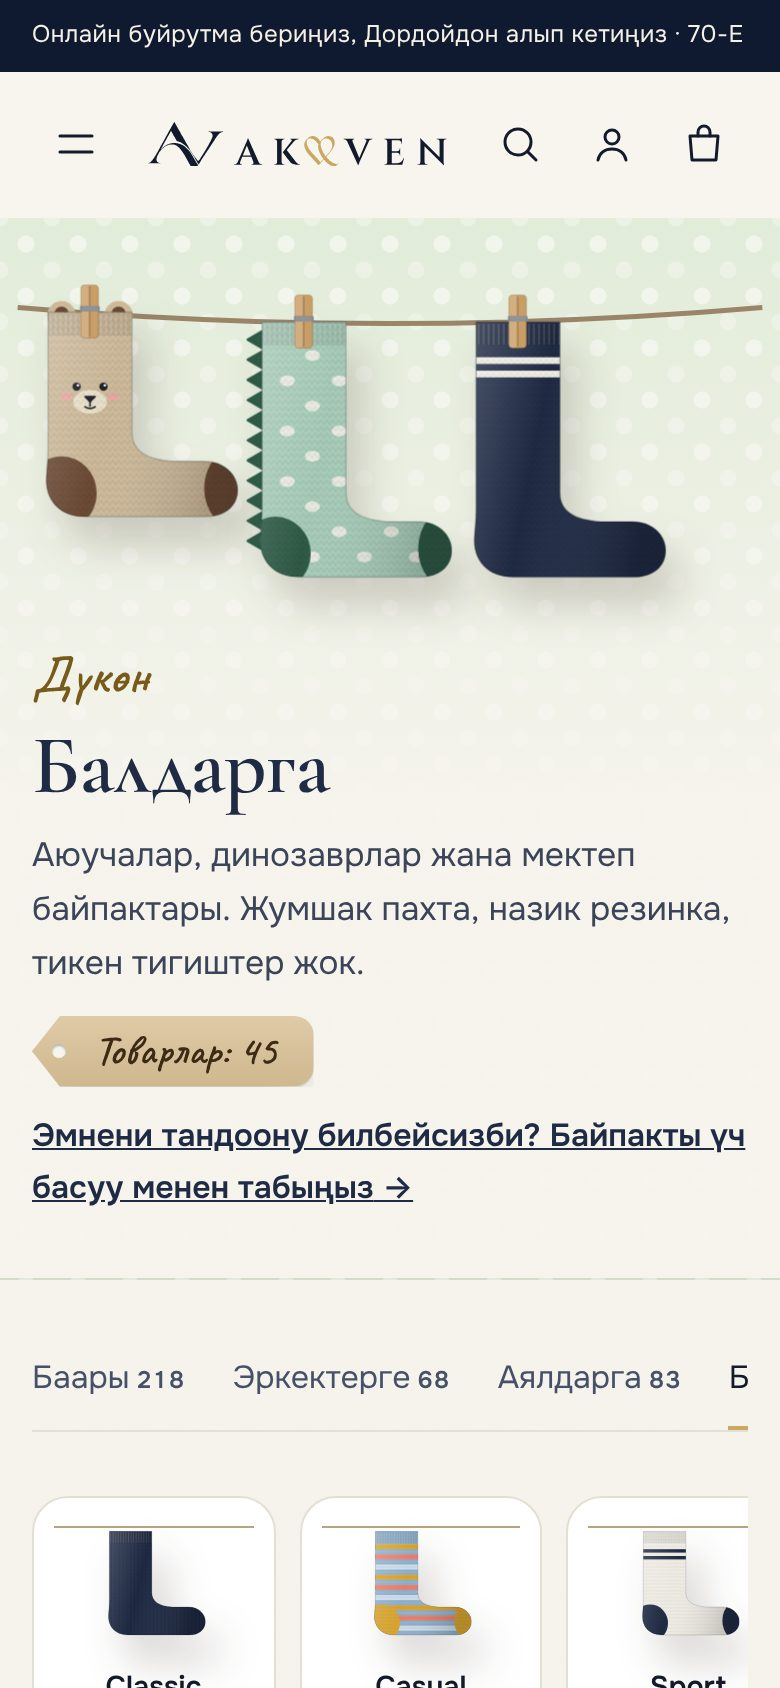
\includegraphics[width=0.38\textwidth,frame]{u-phone-kids-ky.jpg}
	\caption{The home page and the children's shelf on a phone, in Kyrgyz}
	\label{fig:phone}
\end{figure}

\section{The administration}
\label{sec:admin}

The administration is opened at \texttt{/admin} by a staff, owner or super admin account. Its menu (on the left)
groups the screens by who may use them: \emph{Shop} for everyone in the team, \emph{Owners} for the owners and
\emph{System} for the super admin. The language can be switched at the bottom of the menu.

\subsection{For the whole team}

\paragraph{Products.} The list (Figure~\ref{fig:a-products}) can be searched and filtered (in the shop, removed). One
screen (Figure~\ref{fig:a-edit}) adds or edits a product: name, audience, section, cut, description, fabric, quality,
care and origin; its options (colour with swatch, size, pack, price, stock, stock on the way and when it arrives); and
its pictures, each of which can belong to one colour. Pictures are uploaded as JPEG, PNG or WebP of up to 5~MB.
Removing a product hides it from the shop; it can be restored. Every change appears in the product's history.

\shot{a-products.jpg}{Products}{fig:a-products}
\shot{a-product-edit.jpg}{Adding a product}{fig:a-edit}

\paragraph{Orders and hand-over.} \emph{Orders} (Figure~\ref{fig:a-orders}) lists the orders by status; a gift order
says how to pack it, a delivery order the area and the fee. An order can be marked as handed over or cancelled (with a
refund). \emph{Hand over an order} (Figure~\ref{fig:a-handover}) is the stall's screen: the customer's code, typed or
scanned from their QR code, and the last four digits of their phone number.

\shot{a-orders.jpg}{Orders}{fig:a-orders}
\shot{a-handover.jpg}{Handing an order over at the stall}{fig:a-handover}

\paragraph{Sections and cuts} are the owners' own groups of the catalogue; they can be added, renamed, hidden,
reordered, and deleted when no product uses them.

\paragraph{Negotiations and the dashboard.} \emph{Negotiations} (Figure~\ref{fig:a-negotiations}) lists every
conversation with what the assistant proposed and what was allowed. The dashboard (Figure~\ref{fig:a-dashboard}) shows
paid orders, revenue and pairs sold per day, orders waiting at the stall, socks running out with what is on the way,
customers waiting for a sold-out option, and for the assistant the offers per day, how often the limit stepped in and how
many offers became orders.

\shot{a-negotiations.jpg}{Negotiations: proposed and allowed, side by side}{fig:a-negotiations}
\shot{a-dashboard.jpg}{The dashboard}{fig:a-dashboard}

\paragraph{Reviews and wholesale requests.} Reviews wait for approval before they are shown. \emph{Wholesale requests}
(Figure~\ref{fig:a-wholesale}) is the inbox of requests from shops and companies, newest first: the reference, the
company, the city, the pairs and the mix, the contact with a \emph{Reply} button that opens the customer's own WhatsApp,
Telegram, phone or e-mail, a note for the family, and the status (new, in progress, answered, closed).

\shot{a-wholesale.jpg}{The inbox of wholesale requests}{fig:a-wholesale}

\subsection{For the owners}

\paragraph{Pricing} (Figure~\ref{fig:a-pricing}) sets the minimum order, the ladder of discounts by pairs, and the som
and rouble rates with their rounding. The limit of each sock (how much it may be discounted at most) and its cost price
are set on the product's options and are visible only to the owners.

\shot{a-pricing.jpg}{Pricing}{fig:a-pricing}

\paragraph{Delivery areas} (Figure~\ref{fig:a-delivery}) are where the shop delivers: for each area the country, a name,
whether it is a courier area or a cargo carrier, the fee in US dollars, the amount from which delivery is free, the
shortest and longest time in days, a note for customers, and for a carrier whether the customer pays it on receipt.
An area can be hidden from checkout or deleted; orders that used it keep their copy.

\paragraph{Emails to customers} lists every email the shop wrote: to whom, about what, in which language, whether it
went out, and the email itself; the order's page shows its own. Without a mail server the page says that the emails are
kept and not sent, and \emph{Send again} delivers one once a server is set up.

\shot{a-delivery.jpg}{Delivery areas}{fig:a-delivery}

\paragraph{Customers, contacts and the stall, and the size chart.} The owners can mark trusted customers, give a
customer a new password or switch a fake account off; enter the contacts shown in the shop and the stall's address and
opening hours; and edit the size chart from which the shop derives every sock size.

\subsection{For the super admin}

\emph{Accounts} adds staff and owner accounts, changes their role, disables them or sets a new password; a disabled
account or a new password ends its sessions at once. \emph{AI assistant} (Figure~\ref{fig:a-assistant}) chooses who
answers the chat (the language model or the rules), shows whether a key is set (never the key itself), offers a box to
try a message, and repeats the evaluation of Section~\ref{sec:evaluation} against the live model. The \emph{Audit log}
(Figure~\ref{fig:a-audit}) shows every change with who made it and the values before and after.

\shot{a-assistant.jpg}{Choosing and trying the assistant}{fig:a-assistant}
\shot{a-audit.jpg}{The audit log}{fig:a-audit}

\section{Troubleshooting}

\begin{description}
	\item[The page shows an older version.] Reload without the cache (Ctrl+Shift+R, or Cmd+Shift+R on a Mac); an
	installed app updates on its next start.
	\item[``Too many attempts'' at sign-in.] After five wrong passwords for an account from one address, sign-in waits
	for fifteen minutes; the message says how long.
	\item[The chat says to wait a little.] A customer can send twenty messages in ten minutes.
	\item[The assistant answers but the language model is not used.] Without \texttt{LLM\_API\_KEY}, or when the model
	does not answer in time, the rules answer; the super admin sees which one answered under AI assistant.
	\item[A delivery country is missing at checkout.] The country has no area shown at checkout; the owners add one under
	Delivery areas.
	\item[The backend does not start.] Check that port 8080 and 5432 are free and that Docker has enough memory; the
	backend log names the reason.
\end{description}

\section{Limitations}

Payment is simulated: no money moves and the wallet does not contact Apple or Google. The shop sends no e-mails or SMS;
customers follow their orders in the account. Product pictures are drawings until the family photographs the real
socks. The section and colour names come from the owners' data and are shown as entered, in one language.
